\documentclass{article}
\usepackage{graphicx}
\usepackage[export]{adjustbox}
\usepackage[a4paper, total={6in, 8in}]{geometry}

%% Path to images
\graphicspath{ {./images/} }

\begin{document}

\title{\vspace{-4cm}Experimental Design for the Testing of a New Golf Ball}
%\title{Experimental Design for the Testing of a New Golf Ball}
\author{Trent Henderson}
\date{}

\maketitle

The golf ball is a critical component of any golfer's equipment setup, but this is especially the case for the modern golfer for whom scientific advancements have been made available. 
Indeed, the impact of experimentation in golf has spread to the academic community, with extensive empirical research existing for a range of facets such as the effects of dimple design on aerodynamics and different synthetic covers on spin rates. 
The remainder of this paper outlines an experimental design for the premier golfing company Titleist to enable rigorous and robust statistical analysis of their upcoming new 2022 season ball.

As a company who are increasingly focused on amateur golfers, Titleist are interested in understanding the performance of their new ball relative to players' existing balls, especially for mid-high handicap players\footnote{The golf handicap system in Australia ranges from 0 to 36, with tiers for "low handicap" including 0-10, "mid handicap" including 11-20, and "high handicap" including 21 and above.}. 
As such, the following research question was developed to guide experimental design: \textit{Does Titleist's new ball design improve spin rates around the green for players who currently play the standard Titleist Pro V1 ball?} 

The proposed study will see each participant hit twenty shots with both their current ball (Titleist Pro V1) and the new ball after hitting fifteen warm up shots prior to formal testing. 
All balls will be mixed in the same bucket and unmarked to avoid any participant equipment bias but electronically marked so that the computer will be able to detect which ball is which.
The response variable \textit{spin rate} will be measured via an advanced launch monitor which can accurately track spin and other statistics for each shot.
Since low handicap players are better players in general, we hypothesise that the new design would make a more marked improvement in spin rates for mid and high (especially high) handicap players who are more reliant on technology to correct mechanical errors in their swing.

It is proposed that a linear model will be fit to the data, with ball type, handicap grouping, and a set of other control variables entered in as predictors. 
An interaction term between ball type and handicap grouping will also be included in addition to the individual main effects. 
Specifically, age (integer, measured in years), sex (categorical, measured as a factor with three levels: Male, Female, Other/Intersex), and stiffness of golf club shaft (categorical, measured as a factor with four levels: Seniors, Regular, Stiff, Extra Stiff) will be entered as covariates to control for extraneous variance. 
Hypothetically, if the research question and hypothesis are supported, results similar to the simulation presented in Figure~\ref{fig:expectations} would be expected.
Here we can see the relative gain in spin rate for the new ball (after controlling for other variables) is much lower for high handicappers, but is quite substantial for mid and especially low handicappers. 
In other words, the new ball's technology may help high handicappers to experience performance closer to those with higher skill.

\begin{figure}[t!]
    \centering
    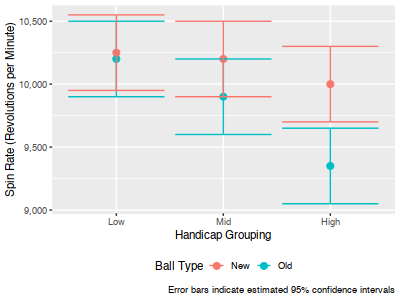
\includegraphics[max width=\linewidth]{expectations}
    \caption{\label{fig:expectations}Hypothesised relationship between ball type and handicap grouping}
\end{figure}

\end{document}